\documentclass[12pt]{article}
\usepackage{graphicx}
\usepackage{epstopdf}
  
%
% Title[Enter title of the experiment here]
\title{EE230: Experiment No.02\\
Zener and BJT Regulator\\}

% Author[Enter details of author here]
\author{Mudavath vishnuvardhan,200070044}

% begin the document.
\begin{document}

% make a title page.[this creates title page]
\maketitle

\section{Overview of the experiment} %[This segment creates Section as seen in document]

\subsection{Aim of the experiment}%[This segment creates sebsections under the same section]

Aim of this experiment is :\\
1.Understanding the limits of performance of a Zener regulator\\
2. Understanding a BJT based series voltage regulator to appreciate the basic blocks of an IC
voltage regulator.

\subsection{ Methods}

I used ngspice software to write code and performed DC analysis for different parameters for zener regulator circuit like changing Load resistance value to 1,10,100,500,1000 ohms and for BJT regulator circuit Load resistance value at 1k ohms and then printed out hardcopy of vout vs vin and currents across different nodes of the circuit , and then extracted output files from each .cir ngspice file in .txt format and then used matplotlib to visualise this data from text file .
\newpage
\section{Design}%[To add multiple sections, keep appending blocks like this]

\subsection{Zener regulator}

\textbf{Case 1: Load resistance (\(R_{l}\))= 1k ohms.\\}
connect a constant 20 volts source with resistances and zener diode as shown below and measure vout at load resistance (\(R_{l}\)).\\
for \(v_{in}=20v\):\\
\(v_{out}= 1.226269*10^{01} V\)\\
\(i_{vs} = 1.646236*10^{-02} A\)\\
\(i_{vze} = 4.199669*10^{-03} A\)\\
\(i_{vl}= 1.226269*10^{-02} A\)\\
Now connect a varying volatage source with resistances and zener diode as shown below and measure vout at load resistance (\(R_{l}\)).
 \begin{figure}[h!]
\centering
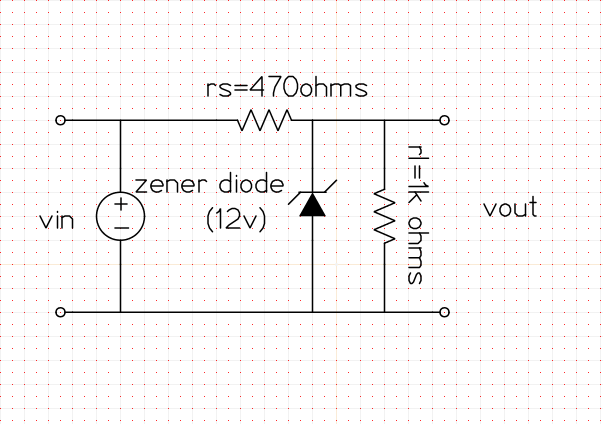
\includegraphics[scale = 0.4]{zener_1k_cir.png}
\end{figure}
\textbf{Case 2: Load resistance (\(R_{l}\))= 500 ohms.\\}
connect a varying volatage source with resistances and zener diode as shown below and measure vout at load resistance (\(R_{l}\)).
 \begin{figure}[h!]
\centering
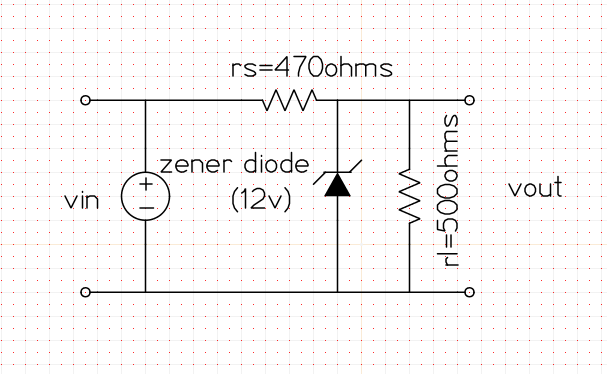
\includegraphics[scale = 0.4]{zener_500_cir.png}
\end{figure}
\newpage

 \textbf{Case 2: Load resistance (\(R_{l}\))= 100 ohms.\\}
connect a varying volatage source with resistances and zener diode as shown below and measure vout at load resistance (\(R_{l}\)).
 \begin{figure}[h!]
\centering
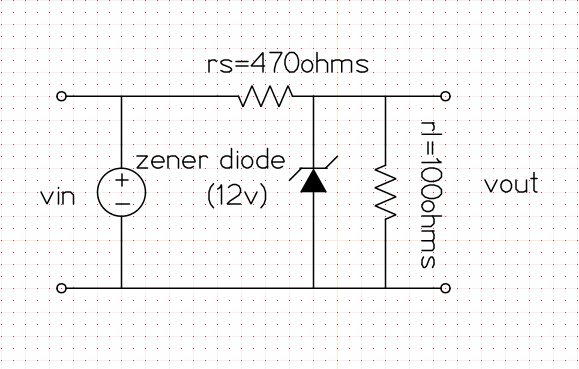
\includegraphics[scale = 0.4]{zener_100_cir.png}
\end{figure}

\textbf{Case 2: Load resistance (\(R_{l}\))= 10 ohms.\\}
connect a varying volatage source with resistances and zener diode as shown below and measure vout at load resistance (\(R_{l}\)).
 \begin{figure}[h!]
\centering
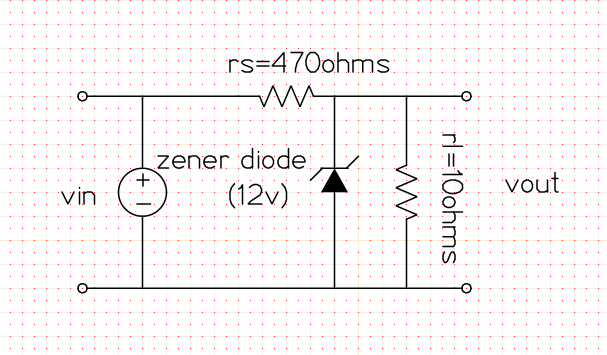
\includegraphics[scale = 0.4]{zener_10_cir.png}
\end{figure}
\newpage
 
 \textbf{Case 2: Load resistance (\(R_{l}\))= 1 ohms.\\}
connect a varying volatage source with resistances and zener diode as shown below and measure vout at load resistance (\(R_{l}\)).
 \begin{figure}[h!]
\centering
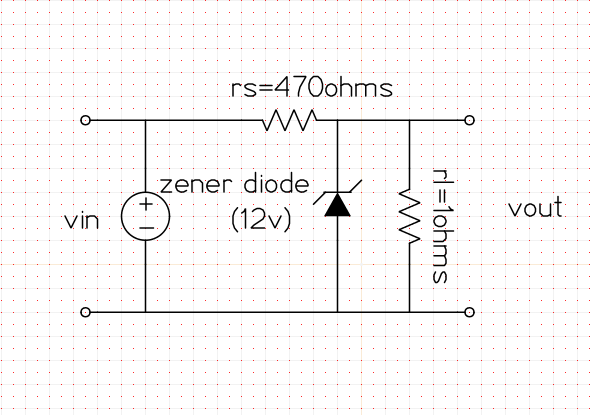
\includegraphics[scale = 0.4]{zener_1_cir.png}
\end{figure}
 \newpage
 
 \subsection{BJT Regulator}
 
\begin{figure}[h!]
\centering
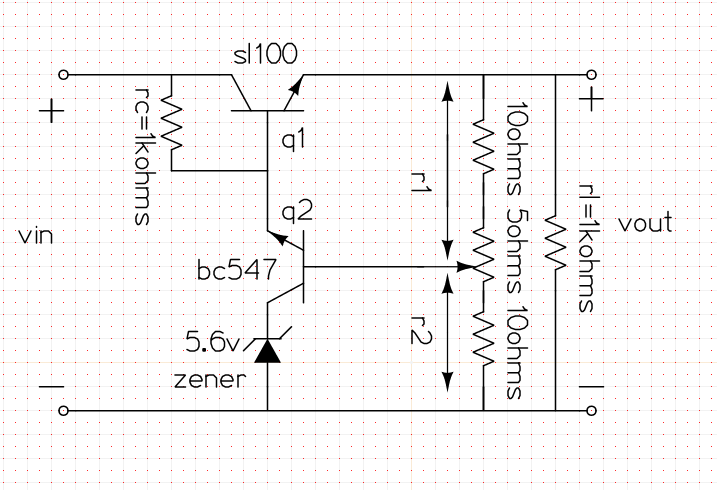
\includegraphics[scale = 0.4]{BJT_reg_cir.png}
\end{figure}

\textbf{Case 1: \(V_{in}\) is 20v , \(R_{1}\) and \(R_{2}\) =12.5v\\}
Connect the circuit as shown above , we get \(v_{out} = 13.78716v\) which is close to theoritical value.

 \textbf{Case 2:\(V_{in}\) is 20v ,\(R_{1}=10.21 k ohms\) and \(R_{2}=14.79 k ohms\)\\}
Connect the circuit as shown above , we get \(v_{out} = 12v\) .

\textbf{Case 3:\(V_{in}\) is varried from 15 v to 25 v and DC analysis is performed in steps of 0.5 v \\}
\newpage
 
 
 
 


 
 
 
 
\section{Simulation results}%[One more section]
\subsection{Code snippet}

\subsubsection{Zener regulator}
\textbf{Case 1: Load resistance (\(R_{l}\))= 1k ohms and \(v_{in}=20v\)\\}
zener regulator\\
.subckt ZENER\_12 1 2\\
d1 1 2 df\\
dz 3 1 dr\\
vz 2 3 10.8\\
.model df D ( IS=27.5p RS=0.620 N=1.10 CJO=78.3p VJ=1.00 M=0.330 TT=50.1n)\\
.model dr D ( IS=5.49f RS=50 N=1.77 )\\
.ends\\
r1  1 2 470\\
vs 2 3 0\\
x1 4 3 ZENER\_12\\
vze 4 0 0\\
r2 3 5 1k\\
vl 5 0 0\\
vin 1 0 20\\
.op\\
.control\\
run\\
print v(2)\\
print v(1)\\
print i(vs)\\
print i(vze)\\
print i(vl)\\
.endc\\
.end\\

\textbf{For other cases only load resistance value r(2) is changed in code for zener regulator and operating point analysis is performed.\\}
\newpage
\textbf{Case 2: Load resistance (\(R_{l}\))= 1k ohms nd \(v_{in}\) varies from 15 to 20v.\\}
zener regulator\\
.subckt ZENER\_12 1 2\\
d1 1 2 df\\
dz 3 1 dr\\
vz 2 3 10.8\\
.model df D ( IS=27.5p RS=0.620 N=1.10 CJO=78.3p VJ=1.00 M=0.330 TT=50.1n)\\
.model dr D ( IS=5.49f RS=50 N=1.77 )\\
.ends\\
r1  1 2 470\\
vs 2 3 0\\
x1 4 3 ZENER\_12\\
vze 4 0 0\\
r2 3 5 1k\\
vl 5 0 0\\
vin 1 0 \\
.dc vin 15 25 0.5\\
.control\\
run\\
print i(vl)\\
plot v(1) v(3)\\ 
plot i(vs) i(vze) i(vl)\\
.endc\\
.end\\
\newpage

\subsubsection{BJT regulator}
\textbf{Case 1: \(V_{in}\) is 20v , \(R_{1}\) and \(R_{2}\) =12.5v\\}
BJT regulator\\
.subckt ZENER\_12 1 2\\
d1 1 2 df\\
dz 3 1 dr\\
vz 2 3 4.4\\
.model df D ( IS=27.5p RS=0.620 N=1.10 CJO=78.3p VJ=1.00 M=0.330 TT=50.1n)\\
.model dr D ( IS=5.49f RS=50 N=1.77 )\\
.ends\\
.include low\_power\_bjt.txt\\
.include sl500\_bjt.txt\\
Q1 1 2 3 SL100	\\
vin 1 0 20\\
rc 1 2 1k\\
r1 3 5 12.5k\\
r2 5 0 12.5k\\
rl 3 0 1k\\
Q2 2 5 4 bc547a\\
x1 0 4 ZENER\_12\\
.op \\
.control\\
run\\
print v(1) v(2)-v(3) v(2)-v(5) v(1)-v(3) v(1)-v(2) v(2)-v(5) v(5)-v(4) v(3)-v(5) v(5)-v(0) v(3)\\
.endc \\
.end\\
\newpage


\textbf{Case 2:\(V_{in}\) is 20v ,\(R_{1}=10.21 k ohms\) and \(R_{2}=14.79 k ohms\)\\}
BJT regulator\\
.subckt ZENER\_12 1 2\\
d1 1 2 df\\
dz 3 1 dr\\
vz 2 3 4.4\\
.model df D ( IS=27.5p RS=0.620 N=1.10 CJO=78.3p VJ=1.00 M=0.330 TT=50.1n)\\
.model dr D ( IS=5.49f RS=50 N=1.77 )\\
.ends\\
.include low\_power\_bjt.txt\\
.include sl500\_bjt.txt\\
Q1 1 2 3 SL100	\\
vin 1 0 20\\
rc 1 2 1k\\
r1 3 5 10.21k\\
r2 5 0 14.79k\\
rl 3 0 1k\\
Q2 2 5 4 bc547a\\
x1 0 4 ZENER\_12\\
.op \\
.control\\
run\\
print v(1) v(2)-v(3) v(2)-v(5) v(1)-v(3) v(1)-v(2) v(2)-v(5) v(5)-v(4) v(3)-v(5) v(5)-v(0) v(3)\\
.endc \\
.end\\



\newpage
\textbf{Case 3:\(V_{in}\) is varried from 15 v to 25 v and DC analysis is performed in steps of 0.5 v and \(R_{1}=10.21 k ohms\) and \(R_{2}=14.79 k ohms\) \\}
BJT regulator\\
.subckt ZENER\_12 1 2\\
d1 1 2 df\\
dz 3 1 dr\\
vz 2 3 4.4\\
.model df D ( IS=27.5p RS=0.620 N=1.10 CJO=78.3p VJ=1.00 M=0.330 TT=50.1n)\\
.model dr D ( IS=5.49f RS=50 N=1.77 )\\
.ends\\
.include low\_power\_bjt.txt\\
.include sl500\_bjt.txt\\
Q1 1 2 3 SL100	\\
vin 1 0 \\
rc 1 2 1k\\
r1 3 5 10.21k\\
r2 5 0 14.79k\\
rl 3 0 1k\\
Q2 2 5 4 bc547a\\
x1 0 4 ZENER\_12\\
.dc vin 15 25 0.5\\ 
.control\\
run\\
print v(3)\\
plot v(1) v(3)\\
.endc \\
.end\\

\newpage


\subsection{Simulation results}
\subsubsection{zener regulator}
\textbf{Case 1: Load resistance (\(R_{l}\))= 1k ohms and \(v_{in}\) varies from 15 to 20v.\\}
X-axis is \(V_{in}\) axis in volts and Y- axis is \(V_{out}\) axis . plot shows linear curve till some point and bends a little.\\
\begin{figure}[h!]
\centering
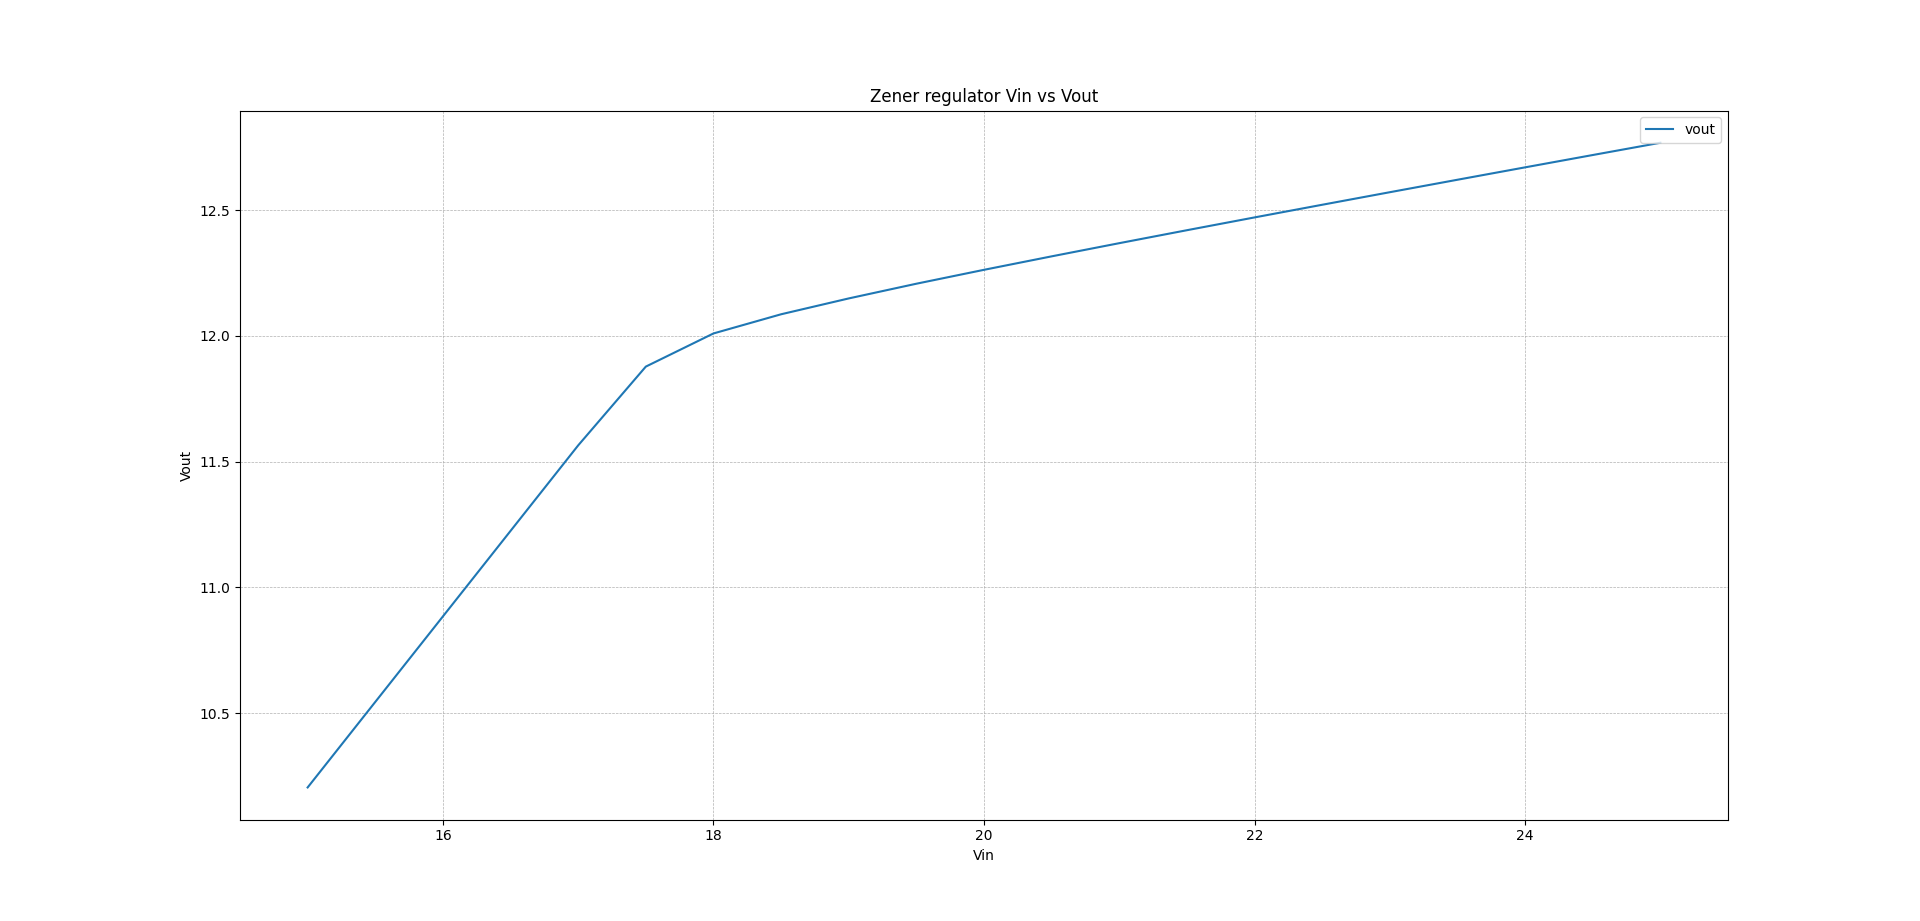
\includegraphics[scale = 0.3]{zener_vin_vout_1k.png}
\end{figure}
\newpage
X-axis is \(V_{in}\) axis in volts and Y- axis is \(I_{rl}\) axis . plot shows linear curve till some point and bends a little.\\
\begin{figure}[h!]
\centering
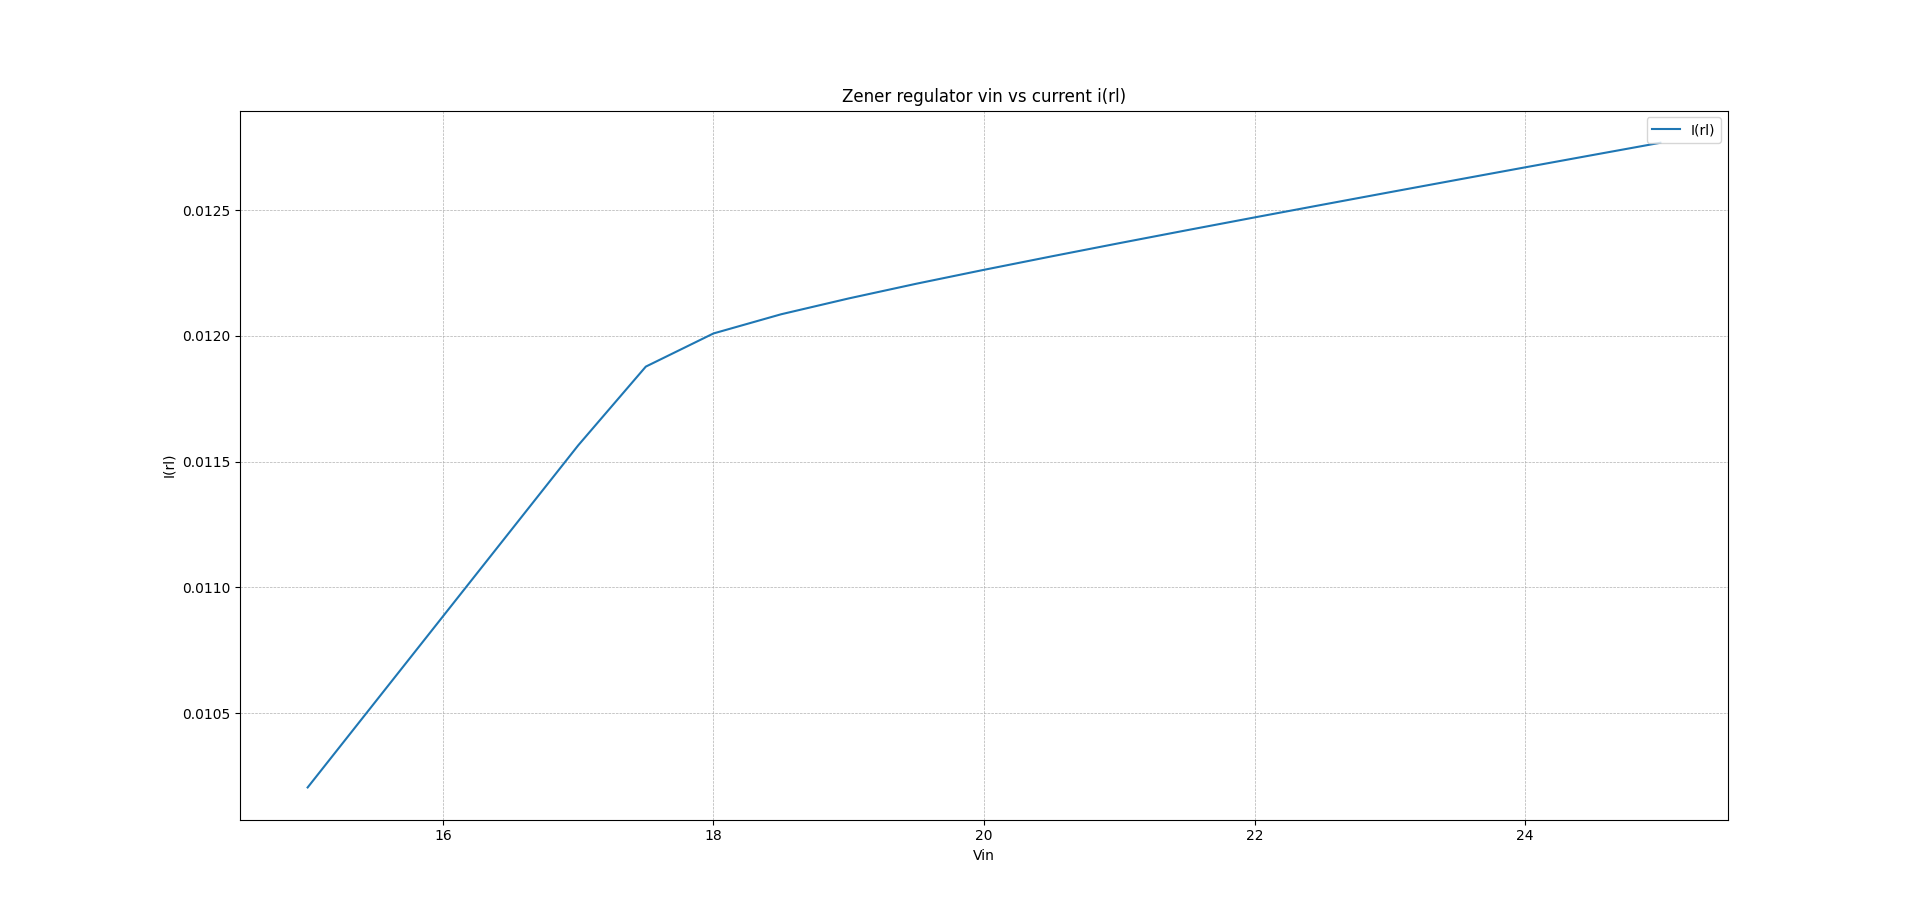
\includegraphics[scale = 0.3]{zener_current_Irl_1k.png}
\end{figure}
\newpage
X-axis is \(V_{in}\) axis in volts and Y- axis is \(I_{rs}\) axis . plot shows linear curve till some point and rises up a little.\\
\begin{figure}[h!]
\centering
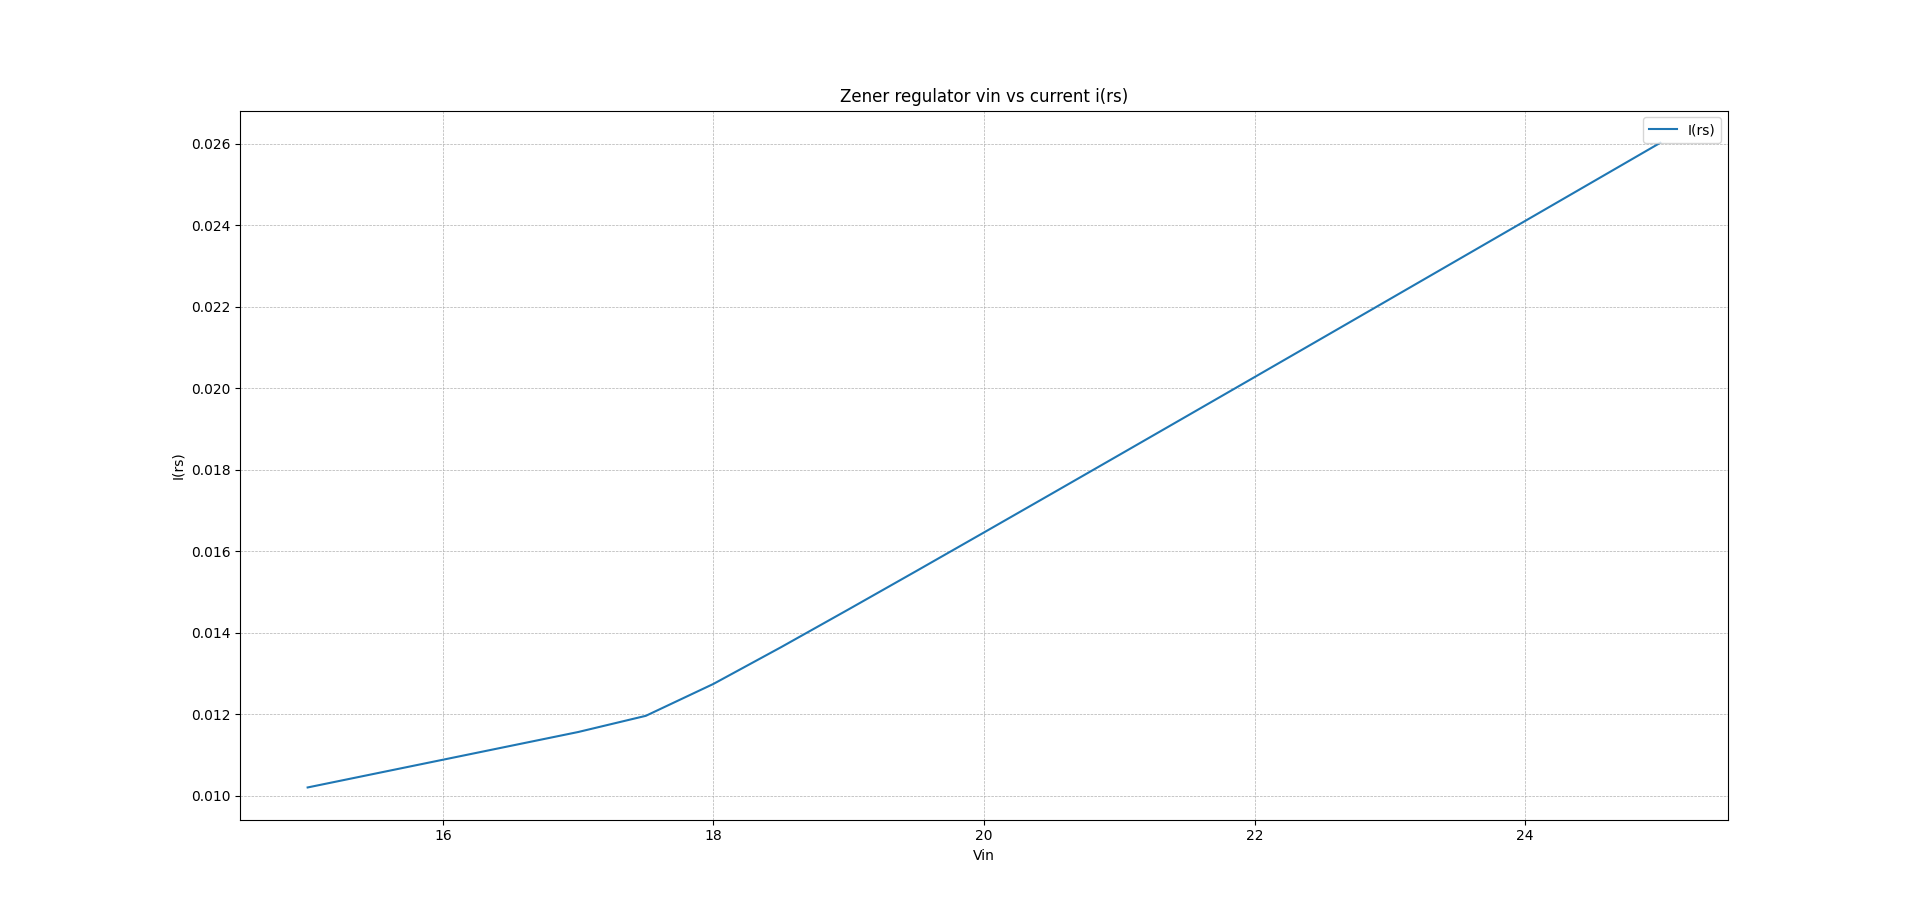
\includegraphics[scale = 0.3]{zener_current_Irs_1k.png}
\end{figure}
\newpage
X-axis is \(V_{in}\) axis in volts and Y- axis is \(I_{z}\) axis . plot shows linear curve till some point and rises up a little.\\
\begin{figure}[h!]
\centering
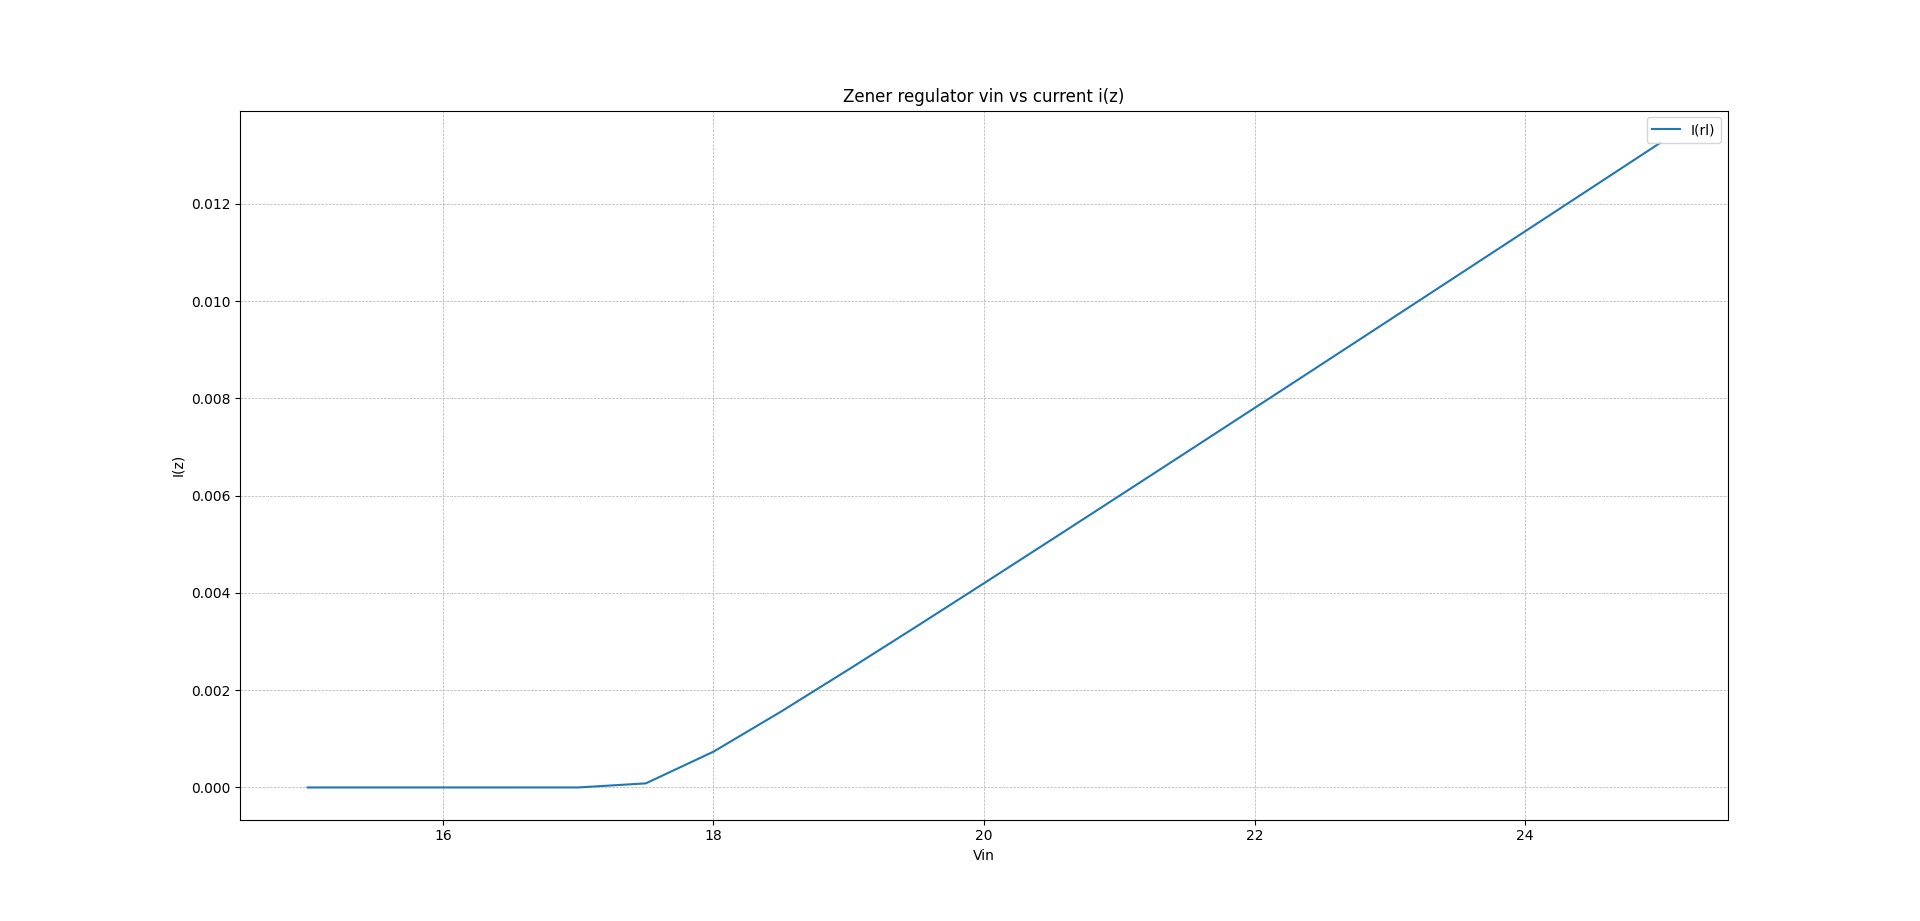
\includegraphics[scale = 0.3]{zener_current_Iz_1k.png}
\end{figure}
\newpage

\textbf{Case 2: Load resistance (\(R_{l}\))= 500 ohms and \(v_{in}\) varies from 15 to 20v.\\}
X-axis is \(V_{in}\) axis in volts and Y- axis is \(V_{out}\) axis . plot shows linear curve till some point and bends a little.\\
\begin{figure}[h!]
\centering
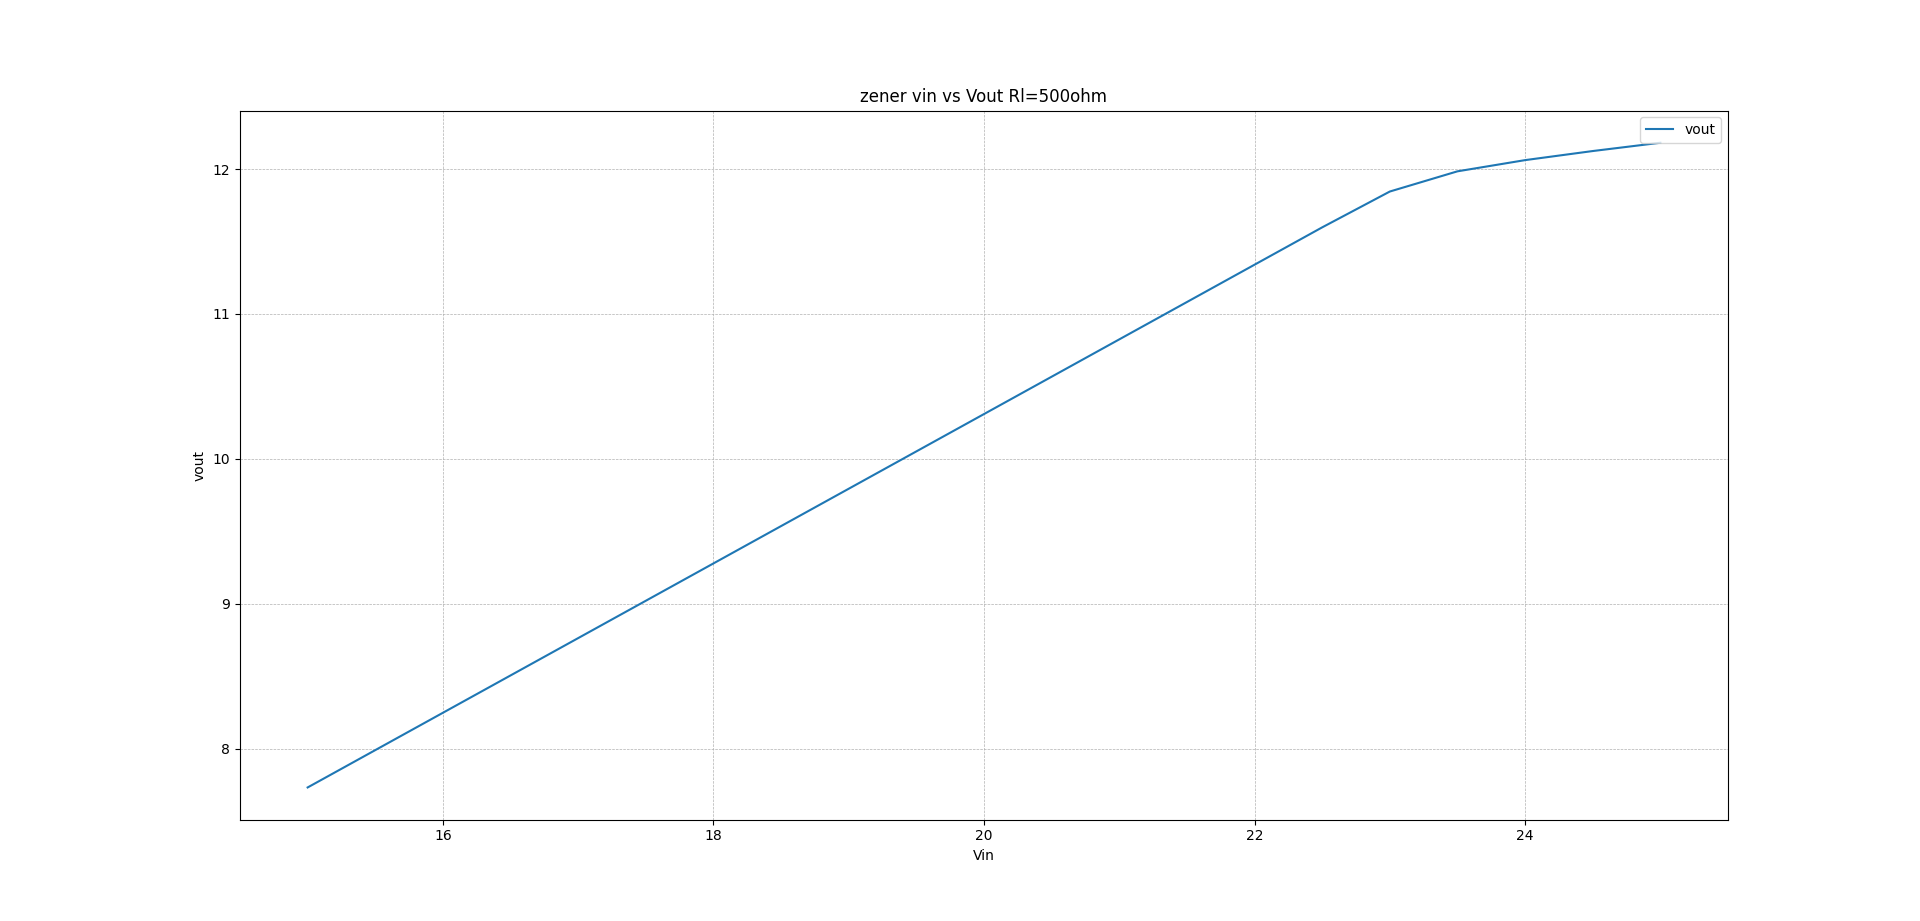
\includegraphics[scale = 0.3]{zener_vin_vout_500.png}
\end{figure}
\newpage

\textbf{Case 3: Load resistance (\(R_{l}\))= 100 ohms and \(v_{in}\) varies from 15 to 20v.\\}
X-axis is \(V_{in}\) axis in volts and Y- axis is \(V_{out}\) axis . plot shows linear curve.\\
\begin{figure}[h!]
\centering
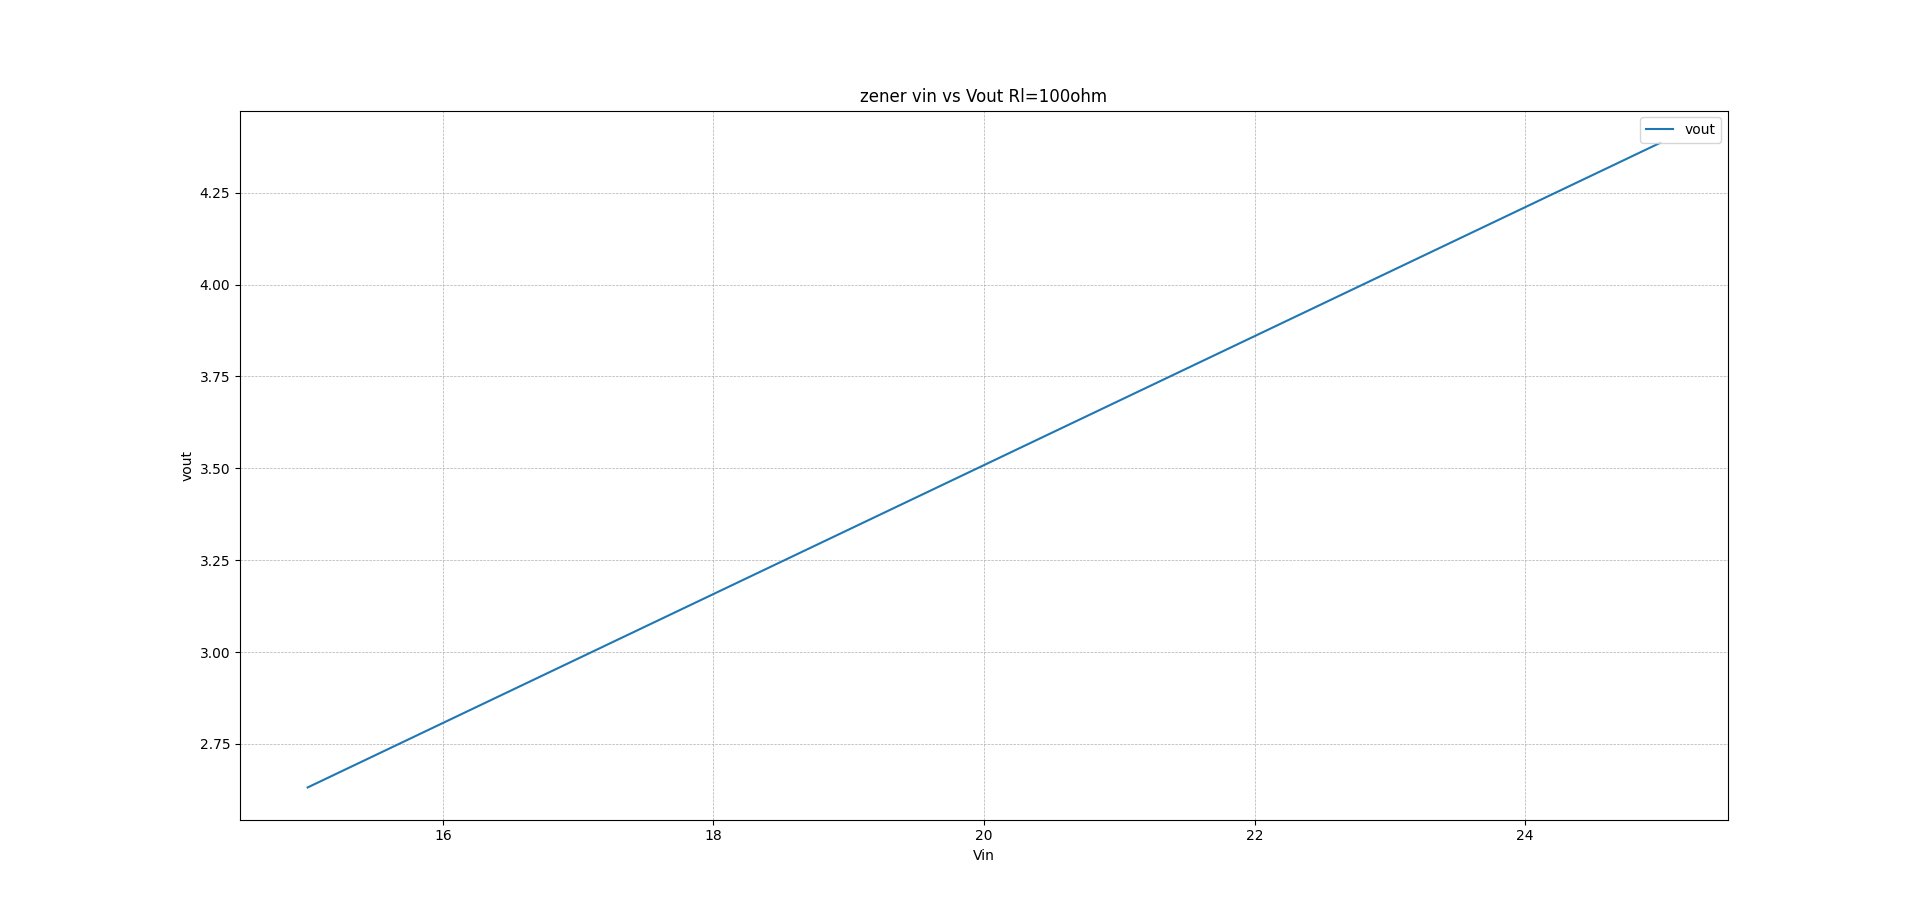
\includegraphics[scale = 0.3]{zener_vin_vout_100.png}
\end{figure}
\newpage

\textbf{Case 4: Load resistance (\(R_{l}\))= 10 ohms and \(v_{in}\) varies from 15 to 20v.\\}
X-axis is \(V_{in}\) axis in volts and Y- axis is \(V_{out}\) axis . plot shows linear curve.\\
\begin{figure}[h!]
\centering
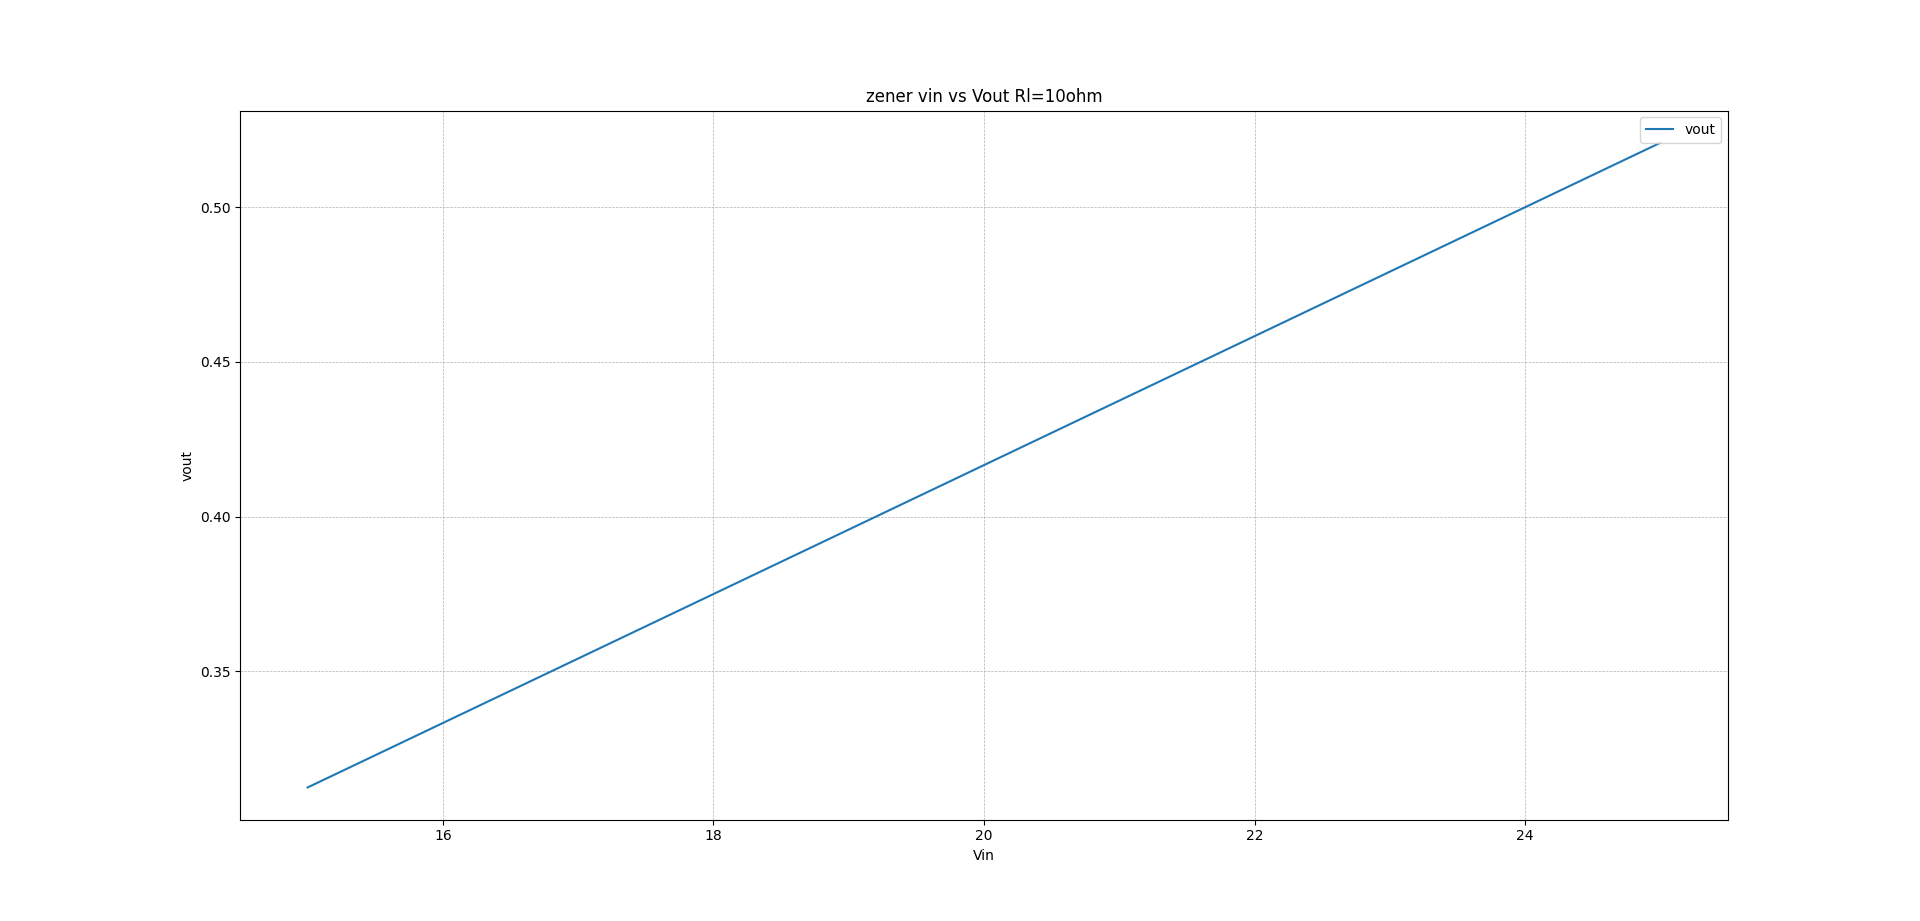
\includegraphics[scale = 0.3]{zener_vin_vout_10.png}
\end{figure}
\newpage

\textbf{Case 5: Load resistance (\(R_{l}\))= 1 ohms and \(v_{in}\) varies from 15 to 20v.\\}
X-axis is \(V_{in}\) axis in volts and Y- axis is \(V_{out}\) axis . plot shows linear curve.\\
\begin{figure}[h!]
\centering
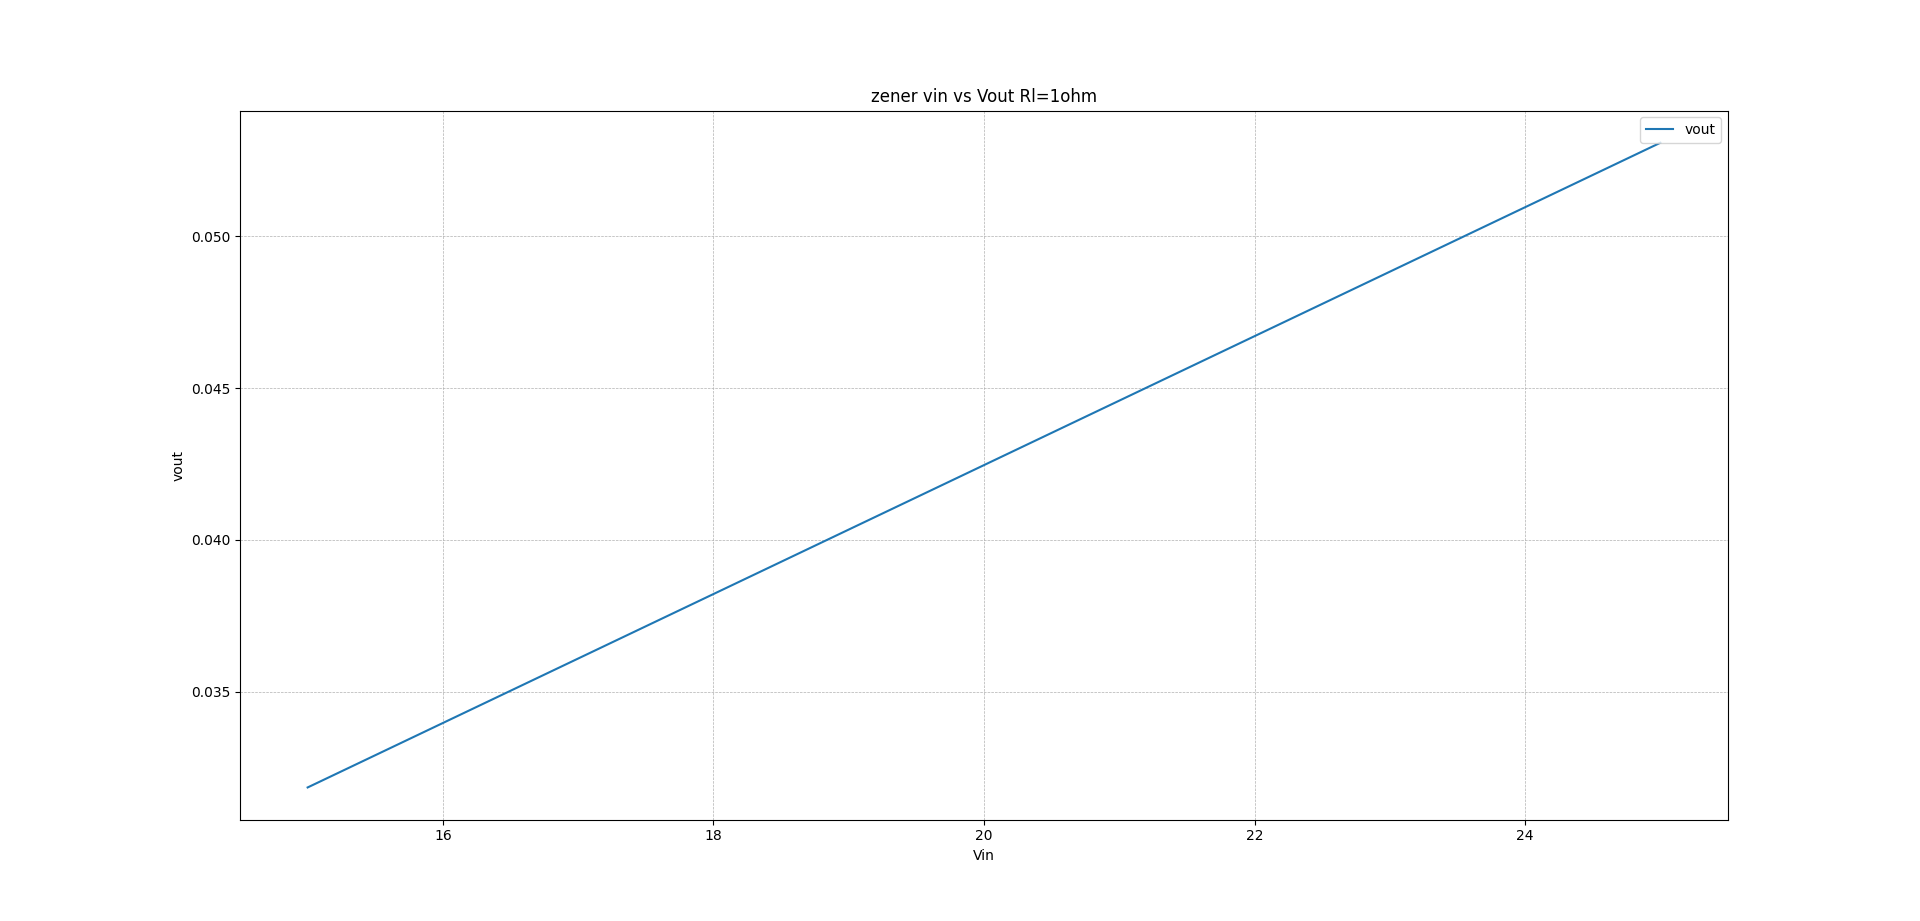
\includegraphics[scale = 0.3]{zener_vin_vout_1.png}
\end{figure}
\newpage

\subsubsection{BJT regulator}


\textbf{Case 1:\(V_{in}\) is varried from 15 v to 25 v and DC analysis is performed in steps of 0.5 v and \(R_{1}=10.21 k ohms\) and \(R_{2}=14.79 k ohms\) \\}
X-axis is \(V_{in}\) axis in volts and Y- axis is \(V_{out}\) axis . plot shows linear curve .\\
\begin{figure}[h!]
\centering
\includegraphics[scale = 0.3]{BJT_vin_vout.png}
\end{figure}
\newpage

\section{Experimental results}
\begin{table}[!hbt]
		% Center the table
		\begin{center}
		\caption{zener regulator voltage and current values for \(v_{in}=20v\) .}
		\begin{tabular}{|c|c|c|c|c|c}
			% To create a horizontal line, type \hline
			\hline
			% To end a column type &
			% For a linebreak type \\
			Sr. No. & Rl=1k ohms & Rl=500 ohms & Rl=100 ohms & Rl=10 ohms & Rl=1 ohms\\
			\hline
			Vout & 12.26269V  & 10.30928V & 3.508772V & 0.4166667V & 0.04246285V \\
			\hline
			Ivs & 0.01646236A & 0.02061856A & 0.03508772A & 0.04166667A & 0.04246285A\\
                       \hline
                       Ivl & 0.01226269A  & 0.02.061856A & 0.03508772A & 0.04166667A & 0.04246285A\\
            
		\end{tabular}
		\end{center}
\end{table}

\section{Experiment completion status}
I have completed all sections in Lab only.

\end{document}
